\documentclass{beamer}
\usetheme{Boadilla}
\usecolortheme{default}
% \usepackage{pgfpages} % TO DELETE
% \setbeameroption{hide notes} % Only slides
% \setbeameroption{show only notes} % Only notes
\setbeameroption{show notes on second screen=right} % Both
\setbeamertemplate{note page}{\pagecolor{yellow!5}\insertnote}\usepackage{palatino}

\usepackage[utf8]{inputenc}
\usepackage[round]{natbib}



\title[Implicit Bias: Rank Min. in ReLU Networks]{Implicit Regularization Towards Rank Minimization in ReLU Networks}
\author[Nadav Timor]{
    by Nadav Timor\newline
    Advisor: Prof. Ohad Shamir
}
\institute[Weizmann Institute]{Weizmann Institute of Science}
\date[January 2022]{January 2022}
\logo{
\includegraphics[height=.75cm]{WeizmannLogo.png}}




\begin{document}



\frame{\titlepage}

\begin{frame}
    \frametitle{Implicit~Regularization Towards Rank~Minimization\\in ReLU~Networks}
    A joint paper under review @ ICML 2022,\\
    w/ Gal Vardi and Ohad Shamir.
\end{frame}



\AtBeginSection[]
{
    \begin{frame}{Table of Contents}
        \tableofcontents[currentsection]
    \end{frame}
}



\section{Introduction}

\begin{frame}{Introduction}{1. Generalization despite overparameterization}
    \newline
    If \#[learnable parameters] $>>$ \#[training examples]:
    \pause
    \begin{columns}
        \column{0.5\textwidth}
        \begin{itemize}
            \item Many global minima\\
            (w/ $0$ training loss). 
            \pause
            \item Might overfit.
        \end{itemize}
        \column{0.5\textwidth}
        \begin{figure}
        \centering
            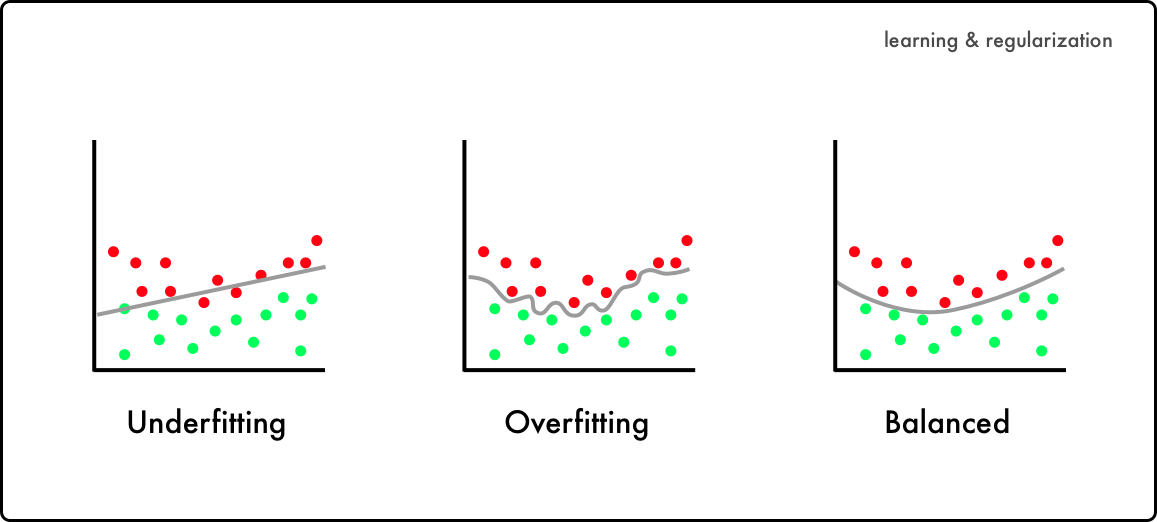
\includegraphics[width=6cm]{figures/overfitting.png}
            % \caption{}
            % \label{fig:overfitting}
        \end{figure}
    \end{columns}
    \pause
    \begin{block}{Phenomenon in practice (\cite{zhang2017understanding})}
        NNs trained \alert{w/o explicit~regularization} generalize well.
        \newline
        \newline
        (despite \#[learnable parameters] $>>$ \#[training examples])
    \end{block}
    \pause
    \begin{itemize}
        \item[Q:] How?\\
        \pause
        \item[Possible A:] Implicit regularization/bias.
    \end{itemize}
    
    \note{
        \begin{enumerate}
            \item \cite{zhang2017understanding}:\\
            Large CNNs, trained w/ stochastic~gradient~methods\\
            fit a random~labeling (of the training~data), or even completely~unstructured random~noise.\\
            Unaffected by explicit~regularization.
        \end{enumerate}
    }
\end{frame}




\section{Results}

\begin{frame}{Sample frame title}

In this slide, some important text will be
\alert{highlighted} because it's important.
Please, don't abuse it.

\begin{block}{Remark}
Sample text
\end{block}

\begin{alertblock}{Important theorem}
Sample text in red box
\end{alertblock}

\begin{examples}
Sample text in green box. The title of the block is ``Examples".
\end{examples}
\end{frame}


\section*{References}
\begin{frame}{References}
    \bibliography{bib}
    \bibliographystyle{abbrvnat}    
\end{frame}

\end{document}